\documentclass[a4paper, amsfonts, amssymb, amsmath, reprint, showkeys, nofootinbib, twoside]{revtex4-2}
\usepackage[spanish]{babel}
\usepackage[utf8]{inputenc}
\usepackage{float}
\usepackage[colorinlistoftodos, color=green!40, prependcaption]{todonotes}
\usepackage{amsthm}
\usepackage{mathtools}
\usepackage{physics}
\usepackage{xcolor}
\usepackage{graphicx}
\usepackage[left=23mm,right=13mm,top=35mm,columnsep=15pt]{geometry} 
\usepackage{adjustbox}
\usepackage{placeins}
\usepackage{lipsum}
\usepackage{csquotes}
\usepackage{xspace}
\usepackage[normalem]{ulem}
%\usepackage{alpha}
\bibliographystyle{plain}

\useunder{\uline}{\ul}{}
\usepackage[pdftex, pdftitle={Article}, pdfauthor={Author}]{hyperref} % For hyperlinks in the PDF
%\setlength{\marginparwidth}{2.5cm}
\begin{document}

%El título del experimento realizado es importante.
\title{Medición del indice de refracción del vidrio usando un interferómetro de Michelson}


\author{Barboza, Jose Maximliano D.\\
Calderon, Angel Guillermo}
\email[Correo ]{maxi.pk.1324@gmail.com}

  
%\author{Second Author}
%\email{Second.Author@institution.edu}

\affiliation{Universidad Nacional de Salta.}

\date{\today} % Si lo dejan vacío no les saldrá fecha. La fecha que se muestra es del día en que se compila.

\begin{abstract}
En esta experiencia mediremos en indice de refracción de una placa de vidrio meidante un inerferomentro de Michelson. 
\end{abstract}

\maketitle

\section{Introducción}

El interferometro de Michelson ha sido durante mucho tiempo un equipo popular en los laboratorios de física. Una de sus aplicaciones es la capacidad medir el índice de refracción o el grosor de una placa de vidrio con precisión. Para esto, se utilizan las franjas de interferencia formadas por la diferencia de camino óptico entre dos haces de luz.

Consideremos una placa de vidrio en uno de los brazos del interferometro de Michelson. Supongamos que el rayo que es normal al espejo forma un ángulo de incidencia $\theta_i$ con la placa. El cambio de fase del rayo al pasar por la placa se puede determinar considerando la configuración geométrica detallada en la figura \ref{img1}.

\begin{figure}[h!]
    \centering
    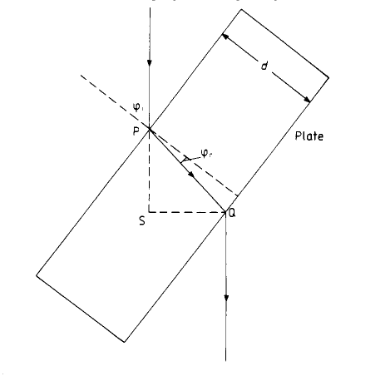
\includegraphics[width=0.8\linewidth]{camino del rayo.png}
    \caption{Detalles de la longitud de camino del rayo a travéz de la placa}
    \label{img1}
\end{figure}

\textbf{Cambio de fase del rayo}

El cambio de fase del rayo al pasar de un punto $P$ a un punto $Q$ se puede expresar como:

\begin{equation}
\Delta \phi_{\mathbf{PQ}} = \frac{2\pi n d}{\lambda \cos{\theta_r}}
\end{equation}

donde $\lambda$ es la longitud de onda de la luz monocromatica, $n$ es el indice de refracción del vidrio, $d$ es el grosor de la placa, y $\theta_r$ es el angulo de refracción, con $\sin{\theta_i}=n \sin{\theta_r}$, donde $\theta_i$ es el ángulo de incidencia.

El rayo equivalente en el otro brazo del interferometro pasa a través de una correspondiente cantidad de aire, sufriendo un cambio de fase

\begin{equation}
    \Delta\phi_{\mathbf{PS}}= \frac{2\pi d \cos{(\theta_i -\theta_r)}}{\lambda \cos{\theta_r}}
\end{equation}

Por lo tanto, la diferencia de fase entre los dos rayos es:

\begin{equation}
    \Delta = 2\left(\frac{2\pi n d}{\lambda \cos{\theta_r}} - \frac{2\pi d \cos{(\theta_i -\theta_r)}}{\lambda \cos{\theta_r}}\right)
\end{equation}

Cuando la placa de vidrio es normal al haz ($\theta_i=\theta_r = 0$) la diferencia de fase queda:

\[\Delta_0 = 2\left(\frac{2\pi n d}{\lambda}-\frac{2\pi d}{\lambda}\right)\]

Al girar la placa desde la posición normal a través del ángulo $\theta_i$, el cambio en la diferencia de fase entre los dos rayos es $\Delta - \Delta_0$. Esto corresponde a $m$ franjas, donde $\Delta -\Delta_0 = 2\pi\, m$, y

\begin{equation}\label{ec4}
m = \frac{2d}{\lambda}\left[n\left(\frac{1}{\cos \theta_r} -1\right)+1 - \frac{\cos (\theta_i -\theta_r)}{cos \theta_r}\right]
\end{equation}

Si se conoce $n$, $d$ se puede encontrar a partir de la ecuación (\ref{ec4}) inmediatamente. Si se conoce $d$ pero no $n$, no es posible reorganizar la ecuación (\ref{ec4}) para dar una solución para n ya que $\theta_r$, que depende de $n$, es desconocido. Sin embargo, se puede usar un programa que ajuste de los datos experimentales ($\theta_i$ y $m$) y de esa manera estimar el valor del $n$.

\section{Procedimiento}
La disposición experimental se muestra en la figura (\ref{fig1}). Se utilizó el interferómetro de precisión OS- 9255A \cite{pasco}. La placa es de vidrio estándar de espesor $d=(0.0074 \pm 0.0002)m$. Dicha placa está sobre un soporte que permite girarla, a partir de un transportador (en grados). Se asumió que  $0^{\circ}$ corresponde a la placa normal al haz de incidencia ($\theta_i = \theta_r$), aunque se debería hacer una comprobación de esto usando una escuadra. El láser posee una longitud de onda $\lambda = 632.8 nm$ 

\begin{figure}[h!]
\centering
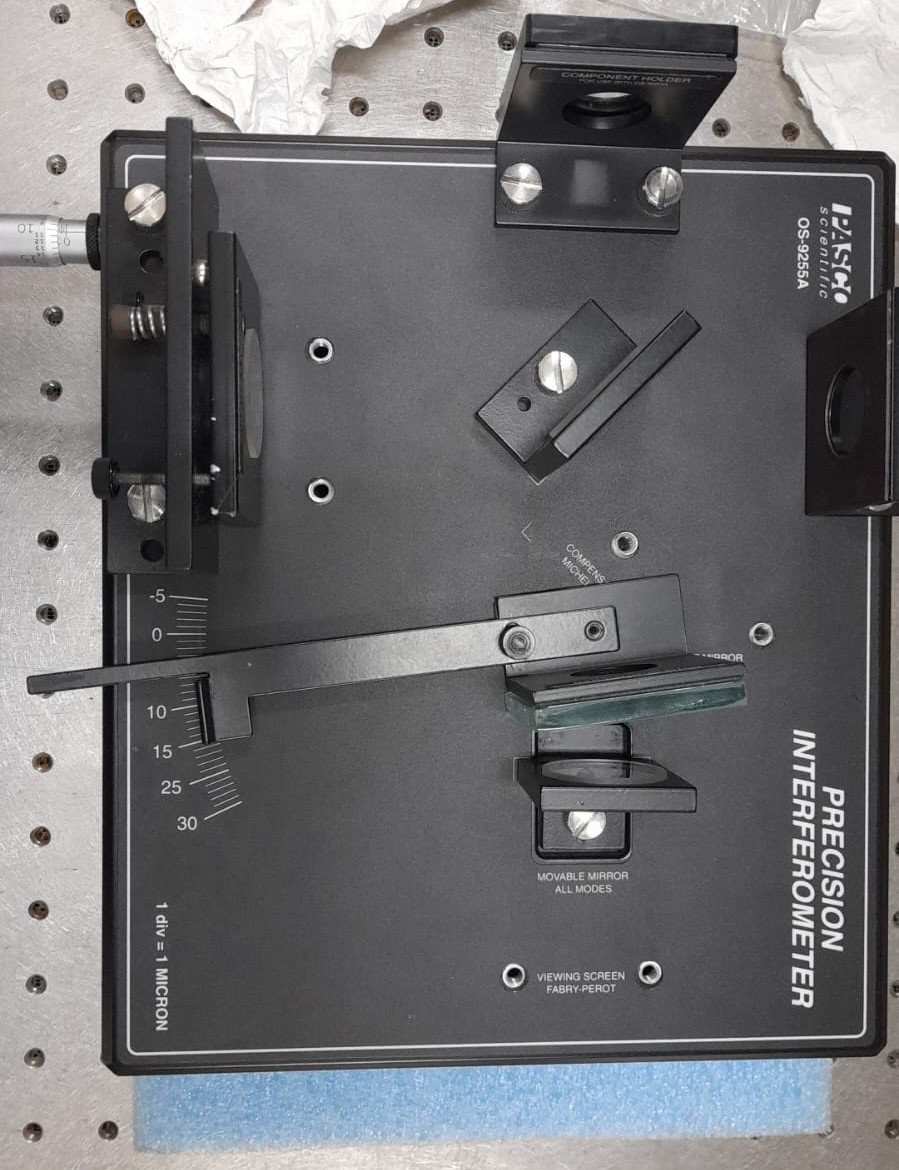
\includegraphics[scale=0.3]{img1.jpeg}
\caption{interferómetro de precisión OS-9255A}\label{fig1}
\end{figure}

Después de calibrar los instrumentos y armar las disposición experimental, con la mano ajustamos el ángulo de incidencia $\theta_i$ girando el soporte y se registra la cantidad de máximos $m$ observados (ver figura \ref{ajuste}). El criterio de medición que se usó es este: se hace girar una cantidad fija el soporte, cada un grado. Y luego se observa cuantos máximos pasaron, en algunos casos no cae en un máximo completo, por lo que agregamos o restamos 0.5 franjas.

En total, se realizaron nueve mediciones de $\theta_i$, con un error $\Delta_{\theta} = 1^{\circ}$, y $m$ con un error de $\Delta_m = 0.5$ ya que se podía observar las franjas entre un mínimo y un máximo. 

Para el calculo del indice de refracción $n$ se usó un ajuste de curva de la ecuación (\ref{ec4}) mediante un programa en Python (curve fitting) \cite{code}. Se obtuvo un $n_{vidrio} = 1.5004$ (figura \ref{ajuste}). Para evaluar la bondad del ajuste entre los datos observados y la curva teórica, se obtuvo un $R^2 = 0.9893$


\begin{figure}[h!]
\centering
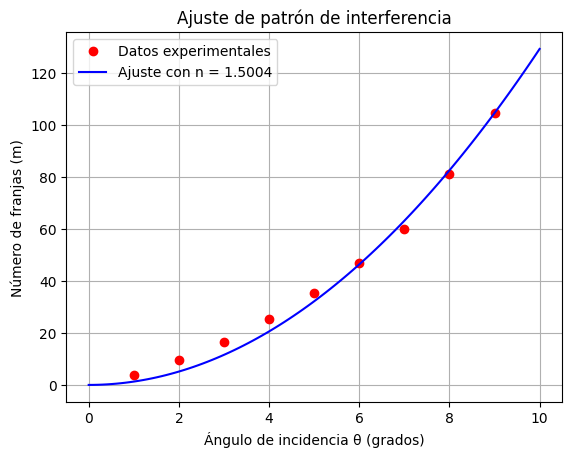
\includegraphics[scale=0.5]{ajuste.png}
\caption{Ajuste de datos para calcular n}\label{ajuste}
\end{figure}

\section{Apéndice de cálculo de errores}

Teniendo en cuenta los errores de apreciación tanto en el espesor del vidrio $d$ como en el ángulo de incidencia $\theta_i$ y el número de máximos $m$, se realiza una propagar el error en el índice de refracción $n$. Entonces, se aplica una variación en cada una de estas magnitudes y se observa cómo afectan al valor ajustado de $n$.

Por ejemplo, para el error en $n$ debido a la incertidumbre en $d$ se ajusta el índice de refracción $n$ utilizando dos valores diferentes de $d$: uno aumentando la incertidumbre $(d+\Delta d)$ y otro reduciendo (minus) en la misma cantidad $(d-\Delta d)$. Luego, se compara la diferencia entre estos dos valores ($n_{plus}$ y $n_{minus}$) para estimar cómo varía $n$ debido a la incertidumbre en $d$. De la misma manera se hace este procedimiento para las demás magnitudes. 

Finalmente, el error total en $n$ debido a $d$, $\theta$, y $m$ se puede combinar usando la fórmula estándar de propagación de errores:

\begin{equation}
\Delta n_{total} = \sqrt{(\Delta n _d)^2+(\Delta n _{\theta})^2+(\Delta n _m)^2}
\end{equation}

El resultado obtenido es:

\[n_{vidrio} = (1.5\pm 0.2)\]

El método curve fitting nos permitió obtener un valor estimado del indice de refracción del vidrio bastante satisfactorio y consistente con valores tabulados, lo que valida la eficacia de nuestro enfoque experimental y el análisis de datos.

\begin{thebibliography}{99}
\bibitem{pasco} PASCO scientific, {\it Instruction Manual and Experiment
Guide for the PASCO scientific Models OS-9255A thru
OS-9258A}, PASCO scientific (2024), accedido: 24-sep-
2024.
\bibitem{michelson}  {\it Measurement of refractive index using a Michelson interferometer}. https://iopscience.iop.org/article/10.1088/0031-9120/17/5/001.
\bibitem{code} {\it Programa de ajuste de datos} https://github.com/angel-calderon-1321/OpticaLab/blob/main/Medici%C3%B3n_del_indice_de_refracci%C3%B3n.ipynb
\end{thebibliography}

\end{document}
